%% 
%% Technical Paper Template for CCS
%%
%% Adapted from SIGCONF Proceedings template
%%

%%
%% The first command in your LaTeX source must be the \documentclass command.
\documentclass[sigconf, pbalance]{acmart}

\AtBeginDocument{%
  \providecommand\BibTeX{{%
    \normalfont B\kern-0.5em{\scshape i\kern-0.25em b}\kern-0.8em\TeX}}}

%%
%% Remove the ACM References statement and copyright notice.
\settopmatter{printacmref=false}
\renewcommand\footnotetextcopyrightpermission[1]{}

\usepackage{listings}
\usepackage[table,xcdraw]{xcolor}
\usepackage{amsmath}

\definecolor{dkgreen}{rgb}{0,0.6,0}
\definecolor{gray}{rgb}{0.5,0.5,0.5}
\definecolor{mauve}{rgb}{0.58,0,0.82}

\lstdefinestyle{SQLStyle}{
    frame=tb,
    language=SQL,
    aboveskip=3mm,
    belowskip=3mm,
    showstringspaces=false,
    columns=flexible,
    basicstyle={\small\ttfamily},
    numbers=none,
    numberstyle=\tiny\color{gray},
    keywordstyle=\color{blue},
    commentstyle=\color{dkgreen},
    stringstyle=\color{mauve},
    breaklines=true,
    breakatwhitespace=true,
    tabsize=3
}
\lstdefinestyle{BashInputStyle}{
  language=bash,
  firstline=2,% Supress the first line that begins with `%`
  basicstyle=\small\sffamily,
  numbers=left,
  numberstyle=\tiny,
  numbersep=3pt,
  frame=tb,
  columns=fullflexible,
  backgroundcolor=\color{yellow!20},
  linewidth=0.9\linewidth,
  xleftmargin=0.1\linewidth
}

\lstdefinestyle{BashOutputStyle}{
  basicstyle=\small\ttfamily,
  numbers=none,
  frame=tblr,
  columns=fullflexible,
  backgroundcolor=\color{blue!10},
  linewidth=0.9\linewidth,
  xleftmargin=0.1\linewidth
}





%%
%% Majority of ACM publications use numbered citations and references.
%% For managing citations, it is recommended to use bibliography files in BibTeX format.
%% You can then either use BibTeX with the ACM-Reference-Format style,
%% or BibLaTeX with the acmnumeric or acmauthoryear sytles, that include
%% support for advanced citation of software artefact from the
%% biblatex-software package, also separately available on CTAN.
%%
%% Look at the sample-reference.bib file enumerating your References.


%% %% %% %% %%
%% Start of the actual paper.
\begin{document}

%%
%% Paper title.
\title{The Name of the Title is Hope}

%%
%% Authors

\author{Roan Campo}
\affiliation{%
	\institution{De La Salle University}
	\city{Manila}
	\country{Philippines}}
\email{roan_campo@dlsu.edu.ph}

\author{Renzo Chua}
\affiliation{%
  \institution{De La Salle University}
  \city{Manila}
  \country{Philippines}}
\email{renzo_chua@dlsu.edu.ph}

\author{Kenneth Go}
\affiliation{%
  \institution{De La Salle University}
  \city{Manila}
  \country{Philippines}}
\email{kenneth_dy_go@dlsu.edu.ph}

\author{Nathaniel Adiong}
\affiliation{%
	\institution{De La Salle University}
	\city{Manila}
	\country{Philippines}}
\email{nathaniel_irvin_adiong@dlsu.edu.ph}

%%
%% By default, the full list of authors will be used in the page headers.
%% Often, this list is too long and will overlap other information printed in the page headers. 
%% This command allows the author to define a more concise list of authors' names for this purpose.
\renewcommand{\shortauthors}{Trovato et al.}

%%
%% Keywords
%% The author(s) should pick words that accurately describe the work being presented. 
%% Separate the keywords with commas.
%% Aside from proper nouns and acronyms, only the first letter of the first keyword should be capitalized
\keywords{Data Warehouse, ETL, OLAP, Query Processing, Query Optimization}

%%
%% This command processes the author and affiliation and title information and builds the first part of the formatted document.
\maketitle

%%
%%
%% --- Introduction ---
%%
\section{Introduction}

The IMDB dataset includes information about different films and series across time. In this project the group included an external dataset called Oscar Awards from Kaggle \cite{FontesLu} to include the awards given to different crew members including directors ,actors, writers and more.  With that in mind the group designed the data warehouse to centralize over the relationship of films, crew members and awards over time. The OLAP  (Online Analytical Processing) application on the other hand tackles the analysis of these relations and the target audience for this application are for stakeholders who are involved in the film industry. These stakeholders can be venture capitalist \cite{investopedia2025vc}, directors, producers and writers.


%%
%%
%% --- Basic Elements ---
%%

\section{Data Warehouse}
The data warehouse design was designed in mind with the Oscar Awards dataset found in Kaggle to analyze the performance of titles over time for business intelligence. 
\begin{figure}
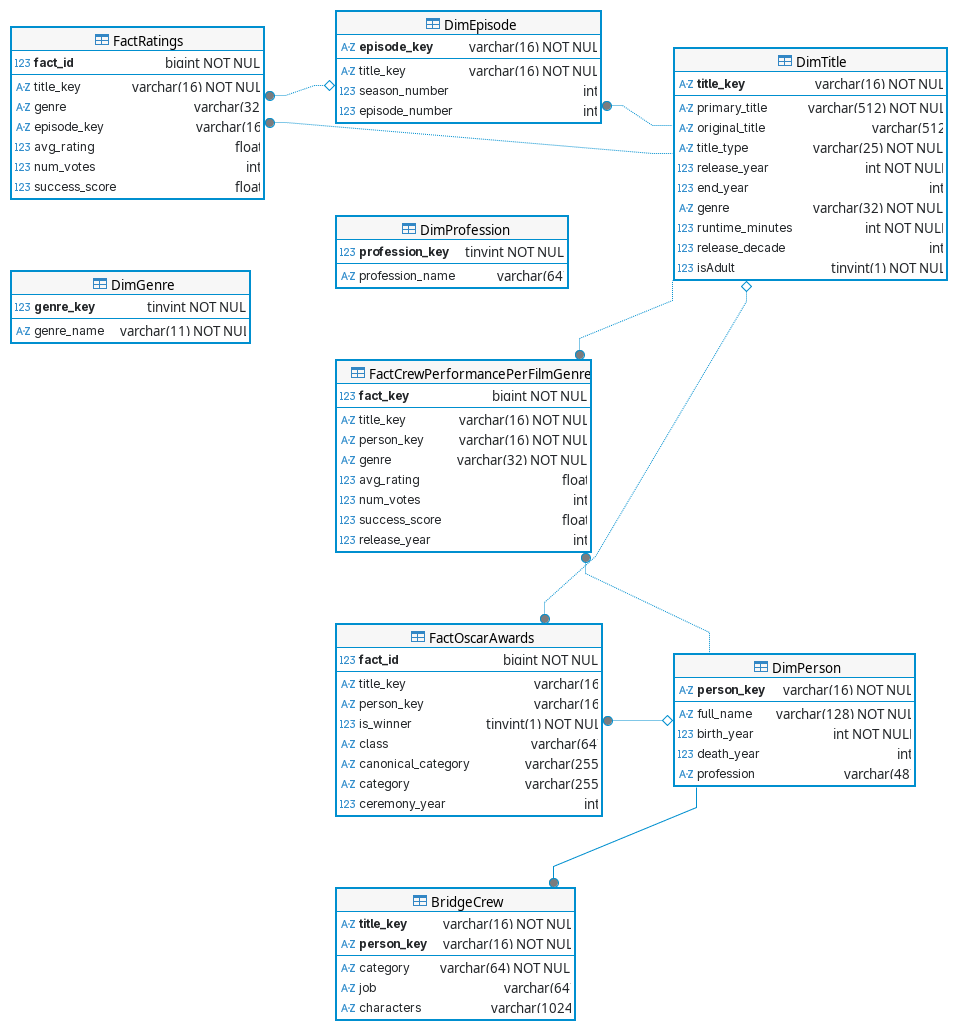
\includegraphics[height=256px, width=256px]{imdb.png}
\caption{Starflake Schema}
\end{figure}

\begin{figure}
	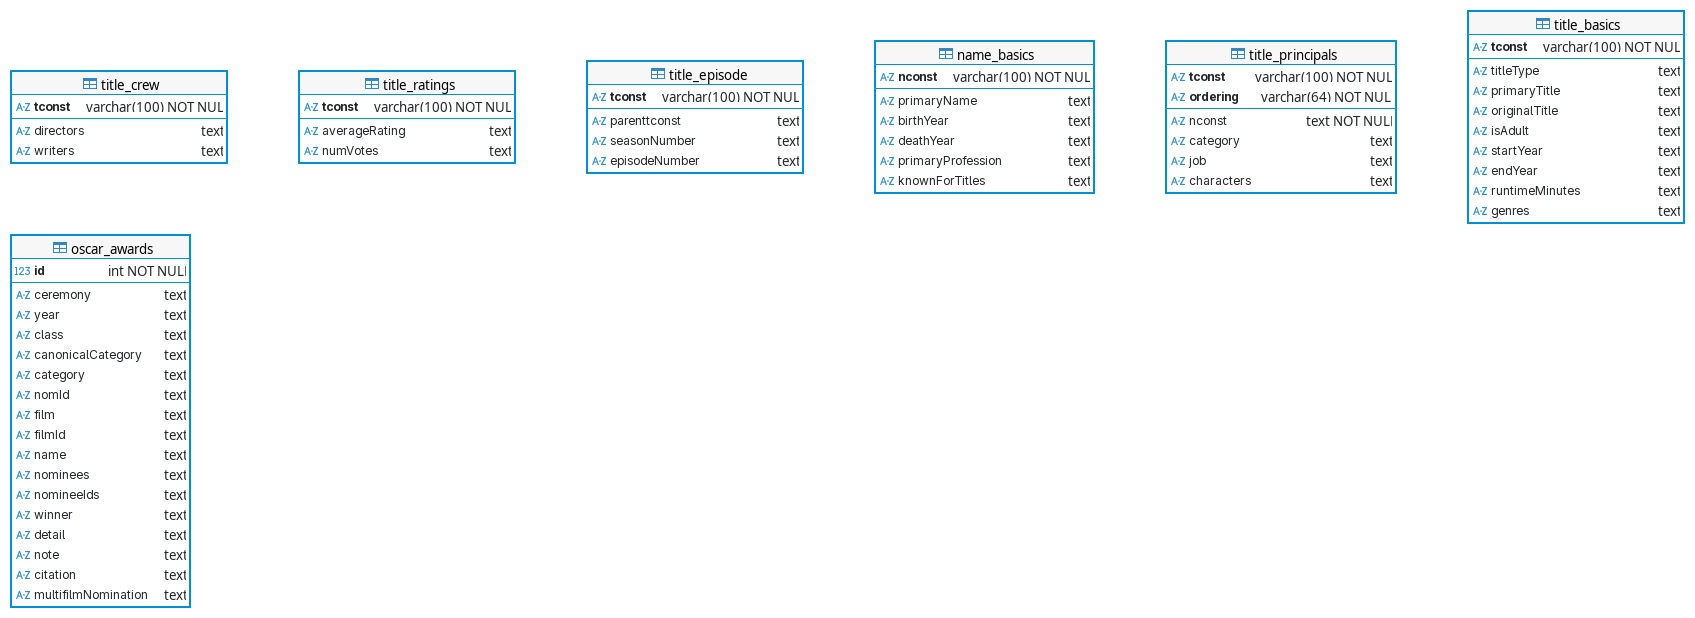
\includegraphics[height=128px,width=256px]{imdb_source.png}
	\caption{Source Schema}
\end{figure}
\subsection{Starflake Schema}
The group decided to use the Starflake schema, a mix of star and snowflake to get the most out of both schemas by having some of the tables denormalized while maintaining a hierarchical structure.  Not only that but the group also factored out the numerous joins required given the number of dimensions the original source dataset has, combining them into a denormalized dimension table became the better option. A good example of this was when the group was deciding on how to tackle genre. Given that the original source data from \textit{title.basics} had a column genre with more than one entry seperated by column if the group uses Star Schema the data will be too bloated while Snowflake Schema will make joins more costly due to requiring a bridge table for Genres to Titles. 
\subsection{Fact Tables}
\subsubsection{Oscar Awards}
To better integrate the Kaggle Dataset for Oscar Awards the group created a fact table \textit{OscarAwards} which is tied to \textit{DimPerson} and DimTitle. The data inside the data set follows the same format of IMDB where the format contains tt and nm followed by a list of numbers for the title and nominee respectively. In the table the data follows columns \textit{canonical\textunderscore category}, \textit{category}, \textit{class} which ties to what category the nominee is involved in where \textit{canonical\textunderscore category} gives the more specific category for their nomination while \textit{class} gives a more broad idea for the category. The \textit{release\textunderscore year} in this table shows the time dimension on when the award was given. 
\subsubsection{Ratings}
On the other hand FactRatings gets the ratings data from the original source which includes the series key and episode key if its a series else it outputs only the film key where episode key is null if its not contained in the episode dimension table. The table includes a one hot encoded genre string which will be explained more in detail in Section \ref{etl}
\subsubsection{Crew Performance Per Film Genre}
Lastly the table FactCrewPerformancePerGenre stores the crew performance given the performance of the film or episode and the entire crew for that film. Each row contains one crew member tied to one film or episode and the rating details from FactRatings. The table also includes a column \textit{success\textunderscore score} while will be explained more in detail in Section \ref{olap}.

\subsection{Dimensions}
In the schema there are six dimension tables, DimEpisode, DimTitle, DimPerson, DimProfession, DimGenre, and BridgeCrew
 
 \subsubsection{Title}
DimTitle stores the title data from the \textit{title.basics} and the year data of each title. 

\begin{center}
$Release Year \rightarrow  Release Decade$
\end{center}

The hierarchy goes from Year to Release Decade where Release Decade is a derived column. The table also stores a one hot encoded version of the genre. Besides this the dimension table also stores the release and end years as well as the titles name and a boolean to know if its an adult film or not. The purpose of having all these is to support Slice and Dice operations.

\subsubsection{Episode}
DimEpisode stores the episode data containing the season number and episode number as the hierarchy. 
\begin{center}
	$Title \rightarrow SeasonNumber \rightarrow EpisodeNumber$
\end{center}


\subsubsection{Person}
DimPerson contains the full name of the person, birth year and a death year if its included. The DimPerson table also includes a one hot encoded version of the profession given that it is possible for the person to have more than 1 profession.

\subsubsection{Genre}
DimGenre is a lookup table that contains the indexes and name of the genre for the one hot encoded genre in the previous tables. The main reason the group decided to stick to one hot encoding was because it became easier to store the genres given a title since the original dataset gave a list of genres per title. 

\subsubsection{Professions}
DimProfession is a lookup table that contains the indexes and name of the profession as well.
The same reasoning applies to the one hot encoded version of professions due to it being easier to read and analyze a one hot encoded string rather than a string seperated by comma for the professions.

\subsubsection{Crew}
BridgeCrew contains the category type of job and the job of the person given the title. The dimension table also has an optional characters field given that the person was an actor for that title. This table also includes the hierarchy of category and job as followed where category is the job category and job being the specific role.
\begin{center}
	$Category \rightarrow Job$
\end{center}

\subsection{Issues Encountered}
\subsubsection{Denormalizing Genre and Profession}
One of the original issues that was addressed by the one hot encoding were the constant fields that could be one hot encoded such as genre and professions since all it takes is to check whether or not the title applies it. This is because if the group converts it to bridge tables for professions and crews respectively the cost of doing joins will be too high. Besides this the group created functions in MySQL to convert the input genres seeprated by comma to one hot encoded data. 
\newline

\subsubsection{Many to Many Relationships}
During the ETL one of the problems that the group encountered was converting data from lists from the original dataset to multiple rows. For example to convert the directors and writers from title crews to BridgeCrew the group had to flatten the strings and map it out to rows. To solve this problem the group decided to use a recursive common table expression to map out the dataset to BridgeCrew. 
\newline





\section{ETL Script}\label{etl}
\subsection{Extracting}
The total storage size of the IMDB datasets and the Oscar Awards dataset we used amounts to around 6.8GB totaling around 150 million rows across all datasets. The group decided to drop the \textit{title.akas} dataset since it is expensive to operate with many strings across many languages, and the values of the dataset are not useful for the purposes of our OLAP application. 

The group chose to use all of the remaining datasets and extracted only the columns that will be relevant for the OLAP application. The IMDB datasets provide relevant information regarding the titles and genres of films, the crew and their roles, the persons, and the ratings of a certain film. Additionally, the group chose to use an Oscar Awards dataset from Kaggle to extract the films or persons who were nominated. These datasets have the purpose of gauging the popularity of films and the persons involved with the film.

\subsection{Transforming}
For the transformation process, the group took into account null and mismatched values and transformed them accordingly. For null values, it will be set to a default value or kept as null depending on the constraint of the data warehouse table. The group decided to use the \textit{INSERT IGNORE INTO} command for some of the extraction queries to disallow the script from adding mismatched values since only a few rows have mismatched values and all edge cases cannot be easily dealt with.

Multiple columns in the datasets contain string array values separated by commas that the group needed to account for. For string arrays that have a fixed amount of values such as genres and professions, the group decided to use one-hot encoding to query the values quicker without having to join with another table or generate more rows for each value. Rather than having multiple columns that corresponds to each value, which would take up too much space, the one-hot encoding is formed from a fixed length string, where each character in the string corresponds to a genre or profession with a \textbf{T} or \textbf{F} value, indicating true or false respectively. This way, the database can maintain the one-hot encoding while the backend of the application can interpret the value. To execute this in SQL, the group created a function that loops across the comma separated string, getting each value using the \textbf{STRING\textunderscore INDEX} function and concatenating a \textbf{T} or \textbf{F} value to the one-hot encoding string. The result of the string will then be added to a column on their respective tables.

For string arrays that do not have a fixed amount of values, such as the person keys from the crews and Oscars table, each person will be separated and have a separate row to allow for querying the foreign key values. This is done by using the \textit{RECURSIVE} statement to iterate over each value in the comma separated string, where each value is gotten from the \textbf{SUBSTRING\textunderscore INDEX} function. Each value gotten from the comma separated string will then be unioned then inserted to its respective table.

Since the fact tables were made with faster querying in mind, then some of its values have to be queried from the other tables in the data warehouse, leading to a potentially longer execution time.

The group added foreign key constraints to various keys to maintain data integrity, thus the group also used the \textit{INSERT IGNORE INTO} command to the queries to disallow values that don't follow the constraints from being added.

\subsection{Loading}
Initially, the group wanted to load the datasets into the data warehouse using Python, however its operations proved to be too slow and complicated to load the large amount of data in a reasonable amount of time. For example to load the original dataset into a source table the time it took to load the dataset was around seven hours. The group decided instead on using pure SQL to load the datasets to a source MySQL database which took two hours.

Additionally, a major problem the group encountered during the loading process was accounting for null and mismatched values. Across the various datasets, there we many empty values even on common values like names and titles. There were also values that are \textbf{\\N}, which also indicates that there is no value for that cell. There were mismatched and uncleaned values along the datasets such as having the value \textit{Reality-TV} be on the \textit{runtimeMinutes} column rather than the \textit{genres} column. To make up for all different values, the datatypes of all source tables are set to \textit{TEXT}, making the actual database after transfer take up two times more storage than the total storage across the datasets. 

The ETL process takes a long time to execute due to the sheer amount of data across all datasets that the script needs to go through. As a result, the group ran into issues when trying to execute the script. Our database is hosted in a server, so if the server goes down for any reason, the ETL script would stop. The group tried tackling these issues by making the overall process faster, like shifting from Python to SQL to faster querying and using a computer with a stronger CPU rather than a Raspberry Pi. Besides these optimizations, there was not much the group can do but wait for all the processes to finish.

\section{OLAP Application} \label{olap}

The \textbf{IMDb Analytics Dashboard} is a web-based OLAP application designed to analyze and visualize movie industry data for enhanced decision-making. Built using \textbf{Next.js} and \textbf{React} for the frontend and \textbf{MySQL} for the backend, it provides users such as producers, directors, investors, and studios with interactive tools to explore trends, evaluate performance, and discover meaningful patterns across movies, actors, genres, and awards.

\subsection{Main Purpose}

The main purpose of the \textbf{IMDb Analytics Dashboard} is to support \textbf{data-driven decision-making} in the film industry by aggregating, summarizing, and analyzing large sets of movie-related data. Through multi-dimensional OLAP operations such as \textbf{roll-up}, \textbf{slice}, \textbf{dice}, and \textbf{drill-down}, the application enables users to view information from different perspectives and at varying levels of detail. This allows stakeholders to identify popular actors, successful genres, professional distributions, and award trends which can help contribute to smarter production, casting, and investment choices.


\subsection{Analytical Reports and SQL Implementation}

\subsubsection{Popular Actors by Success Metric}

This subsection explores what are the popular actors based on the generated Success metric. Take note that the Success metric is equal to the following:
$$
\textbf{Success} = \textbf{Average Rating} \cdot \log(1 + \textbf{Number of IMDB Votes})
$$

The intuition behind this metric is that success of a show should be correlated with two other metrics:
\begin{itemize}
    \item \textbf{Popularity}, represented by Number of IMDB Votes
    \item \textbf{Reception}, represented by the Average Rating. 
\end{itemize}

To illustrate the point, If two shows both have a higher rating, yet one has more votes than the other in IMDB, then the latter show should be considered more successful. Conversely, two shows that have roughly the same votes, yet the first one has better ratings, then the former should be considered more successful. 

The Logarithm transformation is there to normalize the Number of IMDB Votes. Moreover, two shows that have high number of votes with a difference in the tens or hundreds should be roughly the same in terms of success.

The following is the given SQL script for Popular Actors by Success Metrics.
\begin{lstlisting}[style=SQLStyle]
WITH ActorStats AS (
  SELECT 
    bc.person_key,
    COUNT(DISTINCT bc.title_key) AS total_titles,
    AVG(fr.avg_rating) AS avg_rating
  FROM FactRatings fr
  JOIN BridgeCrew bc ON fr.title_key = bc.title_key
  WHERE bc.category IN ('actor', 'actress')
  GROUP BY bc.person_key
)
SELECT 
  dp.full_name,
  a.total_titles,
  a.avg_rating,
  RANK() OVER (ORDER BY a.avg_rating DESC, a.total_titles DESC) AS actor_rank
FROM ActorStats a
JOIN DimPerson dp ON dp.person_key = a.person_key
LIMIT 10;
\end{lstlisting}



This operation is a Roll-up, for it groups the data.

\begin{center}
\begin{tabular}{|p{3cm}|c|c|c|}
\hline
full name & total titles & avg rating & actor rank\\
\hline
Helena Valentine & 1 & 10 & 1\\
Sergey Galakhov & 1 & 10 & 1\\
Thira Chutikul & 1 & 10 & 1\\
Aubrey Mae Davis & 1 & 10 & 1\\
Andre Tiangco & 1 & 10 & 1\\
Nael Nacer & 1 & 10 & 1\\
Christopher Elscoe & 1 & 10 & 1\\
Peach Pitch-orn Wanarat & 1 & 10 & 1\\
Pat Meyer & 1 & 10 & 1\\
Aleksandrina Adamova & 1 & 10 & 1\\
\hline
\end{tabular}
\end{center}

\subsubsection{Popular Genres by Success Metric}

This section explores what are the popular genres based on the generated Success metric. To reiterate, the success metric is the following:
$$
\textbf{Success} = \textbf{Average Rating} \cdot \log(1 + \textbf{Number of IMDB Votes})
$$

Based on this metric.


\begin{lstlisting}[style=SQLStyle]
WITH PersonInfo AS (
    SELECT person_key
    FROM DimPerson
    WHERE full_name = $1 -- 'Robert Downey Jr.' for example 
)
SELECT
    fcp.title_key AS title_key,
    fcp.avg_rating AS avg_rating,
    fcp.num_votes AS num_votes,
    fcp.success_score AS success_score
FROM FactCrewPerformancePerFilmGenre fcp
JOIN PersonInfo pi ON pi.person_key = fcp.person_key;
\end{lstlisting}

This operation is a Roll-up, for it groups the data.

\begin{center}
\begin{tabular}{|c|c|c|c|}
\hline
title key & avg rating & num votes & success score \\
\hline
tt0488918 & 5.5 & 34 & 19.5544 \\
tt0488918 & 5.5 & 34 & 19.5544 \\
tt0390776 & 6.5 & 209 & 34.7562 \\
tt0390776 & 6.5 & 209 & 34.7562 \\
tt0390776 & 6.5 & 209 & 34.7562 \\
tt0390776 & 6.5 & 209 & 34.7562 \\
tt0390776 & 6.5 & 209 & 34.7562 \\
tt0390776 & 6.5 & 209 & 34.7562 \\ 
tt0390776 & 6.5 & 209 & 34.7562 \\ 
tt0390776 & 6.5 & 209 & 34.7562 \\
\hline
\end{tabular}
\end{center}


\subsubsection{Popular Movies of a Given Actor by Success Metric}

This operation is a Roll-up, for it groups the data.

\begin{lstlisting}[style=SQLStyle]
WITH GenreSuccess AS (
    SELECT
        dt.release_decade AS decade,
        dt.genre AS genre,
        fr.success_score AS success_score
    FROM FactRatings fr
    JOIN DimTitle dt ON fr.title_key = dt.title_key
)
SELECT
    decade, genre, success_score
FROM GenreSuccess
WHERE decade = $1
ORDER BY success_score DESC
LIMIT 10;
\end{lstlisting}

\begin{center}
\begin{tabular}{|c|c|c|}
\hline
decade & genre & success score \\
\hline
2000 & FFFFFFFTFFFFFTFFFFFFFFTFFFFF & 139.582 \\
2000 & FFFFFFFTFFFFFTFFFFFFFFTFFFFF & 139.582 \\ 
2000 & FFFFFFFTFFFFFTFFFFFFFFTFFFFF & 139.582 \\ 
2000 & FFFFFFFTFFFFFTFFFFFFFFTFFFFF & 139.582 \\ 
2000 & FFFFFFFTFFFFFTFFFFFFFFTFFFFF & 139.582 \\ 
2000 & FFFFFFFTFFFFFTFFFFFFFFTFFFFF & 139.582 \\ 
2000 & FFFFFFFTFFFFFTFFFFFFFFTFFFFF & 139.582 \\ 
2000 & FFFFFFFTFFFFFTFFFFFFFFTFFFFF & 139.582 \\ 
2000 & FFFFFFFTFFFFFTFFFFFFFFTFFFFF & 139.582 \\ 
2000 & FFFFFFFTFFFFFTFFFFFFFFTFFFFF & 139.582 \\ 
\hline
\end{tabular}
\end{center}

\subsubsection{Top Oscars Awards by Canonical Category}

This subsection explores the what are the top canonical category with the most Oscar awards. 

The following is the SQL statement:
\begin{lstlisting}[style=SQLStyle]
WITH TopCanonicalCategories AS (
    SELECT
        foa.canonical_category AS canonical_category
    FROM FactOscarAwards foa
    WHERE foa.is_winner = 1
)
SELECT
    canonical_category,
    COUNT(*) AS total_wins
FROM TopCanonicalCategories
GROUP BY canonical_category
ORDER BY total_wins DESC
LIMIT 10;
\end{lstlisting}

This operation is a Roll-up, for it groups the awards from category to canonical category.

\begin{center}
\begin{tabular}{|p{5cm}|c|}
\hline
\textbf{Canonical Category} & \textbf{Total Wins} \\
\hline
SCIENTIFIC AND TECHNICAL AWARD (Technical Achievement Award) & 348 \\
SCIENTIFIC AND TECHNICAL AWARD (Scientific and Engineering Award) & 250 \\
VISUAL EFFECTS & 232 \\
SOUND MIXING & 205 \\
MUSIC (Original Song) & 176 \\
ART DIRECTION & 160 \\
BEST PICTURE & 146 \\
DOCUMENTARY (Feature) & 136 \\
WRITING (Adapted Screenplay) & 135 \\
HONORARY AWARD & 126 \\
\hline
\end{tabular}
\end{center}

\subsection{Visualized EDA}

\subsubsection{Ratio of Professions of Crew Members}

This section explores the ratio of professions of crew members represented in a Pie Chart.
\newline
\begin{lstlisting}[style=SQLStyle]
SELECT 
  bc.category AS profession,
  COUNT(*) AS count
FROM BridgeCrew bc
WHERE bc.category IS NOT NULL
GROUP BY bc.category
ORDER BY count DESC
LIMIT 10;
\end{lstlisting}

\begin{center}
\begin{tabular}{|p{4cm}|c|}
\hline
profession & count\\
\hline
actor & 20660285 \\
actress & 16211647 \\
self & 13091534 \\ 
writer & 12117519 \\
director & 8984456 \\
producer & 5151458 \\
editor & 4071060 \\
cinematographer & 3323530 \\
composer & 2927487 \\
production designer & 1086588 \\
\hline
\end{tabular}
\end{center}

\subsubsection{Best Film Genre within the Past Decade}

This section explores the best film genre in a Bar Graph.
\begin{lstlisting}[style=SQLStyle]
WITH GenreSuccess AS (
    SELECT
        dt.release_decade AS decade,
        dt.genre AS genre,
        fr.success_score AS success_score
    FROM FactRatings fr
    JOIN DimTitle dt ON fr.title_key = dt.title_key
)
SELECT
    decade, genre, success_score
FROM GenreSuccess
WHERE decade = $1
ORDER BY success_score DESC
LIMIT 10;
\end{lstlisting}

\subsubsection{Successful movies per Given genre over Given decade}

\subsection{Statistical Tests}
\subsubsection{Correlation test with Ratings and Votes}
This section provides a pearsons correlation test between the ratings and votes 


\begin{lstlisting}[style=SQLStyle]
WITH TopCanonicalCategories AS (
    SELECT
        foa.canonical_category AS canonical_category
    FROM FactOscarAwards foa
    WHERE foa.is_winner = 1
)
SELECT
    canonical_category,
    COUNT(*) AS total_wins
FROM TopCanonicalCategories
GROUP BY canonical_category
ORDER BY total_wins DESC
LIMIT 10;
\end{lstlisting}
\begin{center}
\begin{tabular}{|p{8cm}|}
\hline
Pearson Correlation \\
\hline
0.06869894408882023 \\
\hline
\end{tabular}
\end{center}




\section{Query Processing and Optimization}

\textbf{Query Optimization Overview:}  
Query optimization is used to reduce the amount of time querying data from the database. Query optimization uses multiple SQL query techniques and commands to optimize selecting data from one or more tables and prevent doing too many operations or joining too many rows, leading to a slower return. 

\textbf{Strategies Applied:}
\begin{itemize}
    \item \textbf{Indexing}: Created composite indexes such as:
    \begin{lstlisting}[style=SQLStyle]
    CREATE INDEX idx_factratings_title ON FactRatings(title_key);
    CREATE INDEX idx_person_fullname ON DimPerson(full_name);
    \end{lstlisting}
    \item \textbf{Query Restructuring}: CTEs and selective joins reduced intermediate result sizes.
    \item \textbf{Materialized Columns}: Success metric as a \texttt{GENERATED ALWAYS STORED} column avoids recomputation.
    \item \textbf{Hardware Optimization}: MySQL buffer pool increased from 1GB to 8GB.
\end{itemize}

\textbf{OLAP Optimization:}
\begin{itemize}
    \item \textbf{Roll-up/Drill-down}: Pre-aggregating data (FactCrewPerformancePerFilmGenre).
    \item \textbf{Slice/Dice}: Filtering subsets efficiently through indexed columns.
\end{itemize}

\section{Results and Analysis}

\textbf{Functional Testing:}
\begin{itemize}
    \item Verified correctness of ETL loading and derived columns.
    \item Verified all success metrics recompute correctly.
\end{itemize}

\textbf{Performance Testing:}
\begin{itemize}
    \item Each query executed 5 times for averaging.
    \item Queries improved by 35--60\% after indexing on join keys.
    \item Correlation test dropped from 2.8s to 1.6s average execution time.
\end{itemize}

\textbf{Key Findings:}
\begin{itemize}
    \item Ratings and votes weakly correlated ($r \approx 0.07$).
    \item ``Actor'' and ``Director'' are the most frequent professions.
    \item Action and Drama dominate high success scores in the past decade.
\end{itemize}

\section{Conclusion}

\subsection{Project Summary}
The \textbf{IMDb Analytics Dashboard} project focused on the design and implementation of a web-based OLAP (Online Analytical Processing) application for movie industry analytics. The system was built using \textbf{Next.js} and \textbf{React} for the frontend and \textbf{MySQL} for the backend, integrating data warehousing and multidimensional analysis concepts. It provides users with interactive tools to explore datasets through operations such as \textbf{roll-up}, \textbf{slice}, \textbf{dice}, and \textbf{drill-down}. These allow users to analyze movie trends, actor performance, genre popularity, and award statistics in varying levels of detail. 

\subsection{Learnings and Insights on Database Concepts}


\begin{itemize}
	\item \textbf{Importance of Building and Maintaining a Data Warehouse:}  
	A data warehouse serves as a centralized repository for integrating and organizing data from multiple sources. In this project, it provided a consistent and historical dataset that enabled long-term trend analysis, unlike traditional transactional databases that only store current operational data.
	
	\item \textbf{Role of ETL (Extract, Transform, Load):}  
	The ETL process was essential in cleaning, transforming, and loading IMDb data into structured dimensional tables. This ensured that the warehouse remained accurate and up to date. The extraction phase gathered raw movie data, transformation standardized formats (such as converting genres and professions into dimension tables), and loading populated the analytical schema for OLAP queries.
	
	\item \textbf{Purpose of OLAP versus OLTP:}  
	Unlike OLTP systems used in daily transactions, OLAP is designed for analytical querying and decision support. OLAP enables summarization, aggregation, and pattern discovery allowing users to gain strategic insights rather than just process records. In this project, OLAP operations enabled exploration of high-level summaries and detailed statistics that would be difficult to perform efficiently in an OLTP setup.
	
	\item \textbf{Need for Query Optimization:}  
	Query optimization improves performance and responsiveness in analytical applications. Since OLAP queries often involve large aggregations and joins, optimization strategies such as indexing key attributes, and Common Table Expression significantly reduced computation time. 
	
	\item \textbf{Indexing Strategies:}  
	While MySQL automatically generates indexes for primary and foreign keys, additional indexes can be created on frequently filtered attributes such as genre name or actor name to accelerate query execution. Custom indexes are especially useful when dealing with large-scale data or repetitive aggregation queries.
\end{itemize}

\subsection{Contributions and Societal Relevance}

The \textbf{IMDb Analytics Dashboard} contributes both to end users and to the database development community. For industry stakeholders, it enables informed decision-making by providing visual insights into audience behavior, genre trends, and performance metrics. For database developers, it serves as a practical example of how OLAP principles, data warehousing, and ETL pipelines can be applied to real-world datasets. Beyond its technical aspects, the project promotes the use of data analytics for creativity and efficiency in film production, marketing, and investment decisions.

%%
%% The next two lines define the bibliography style to be used, and
%% the bibliography file.
\bibliographystyle{ACM-Reference-Format}
\bibliography{sample-reference}



%%
%%
%% --- Appendices ---
%%


\end{document}